\section{Experiment 1}\label{exp:1}
This is my starting point \cite{3gpp-ts-22-186,3gpp_ts_26_511_v18_1_0}

Every physical capability of the \gls{rsu} is different from each other in terms of maximum wattage.
When the \glspl{rsu} were stressed based on the amount of vehicles, they have a limit of watts also linked to the CPU consumption.

\begin{table}[htbp]
    \centering
    \caption{Average vehicular counts and power consumption per RSU.}
    \label{tab:rsu-traffic-power}
    \begin{tabular}{|c|cc|cc|}
        \hline
        \textbf{RSU} & \multicolumn{2}{c|}{\textbf{Night (17:00--06:00)}} & \multicolumn{2}{c|}{\textbf{Day (06:00--17:00)}}                        \\
        \cline{2-5}
                     & Vehicles                                           & Power (W)                                        & Vehicles & Power (W) \\
        \hline
        1            & 0                                                  & 59                                               & 4        & 58        \\
        2            & 1                                                  & 55                                               & 7        & 55        \\
        3            & 5                                                  & 56                                               & 23       & 56        \\
        5            & 2                                                  & 51                                               & 7        & 51        \\
        6            & 1                                                  & 60                                               & 5        & 60        \\
        7            & 6                                                  & 61                                               & 16       & 61        \\
        \hline
    \end{tabular}
\end{table}
\begin{table}[!t]
    \centering
    \caption{Location mapping between inductive sensors and \glspl{rsu} to monitor vehicular traffic per \gls{rsu} in the E13 Highway, Antwerp Belgium.}
    \label{tab:location-mapping-rsu}
    \begin{adjustbox}{max width=\columnwidth}
        \begin{tabular}{|l|c|l|l|}
            \hline
            \textbf{\gls{rsu}} & \textbf{Vehicles} & \textbf{RSU Location} & \textbf{Nearest Inductive Sensor} \\
            \hline
            1 & 12 & 51.210575, 4.46655        & 51.21056678, 4.466446158 \\
            3 & 25 & 51.215186667, 4.450568333 & 51.21587307, 4.452993707 \\
            7 & 12 & 51.210616667, 4.480896667 & 51.21066931, 4.480559376 \\
            8 & 26 & 51.211091667, 4.491425    & 51.21127494, 4.491424033 \\
            4 & 16 & 51.21574, 4.457151667     & 51.21577734, 4.457154961 \\
            6 & 16 & 51.211236667, 4.472586667 & 51.21121407, 4.472483657 \\
            \hline
        \end{tabular}
    \end{adjustbox}
\end{table}

Table~\ref{tab:rsu-max-capacity} summarizes the maximum number of users (U) and the corresponding maximum wattage (W) capacity for each \gls{rsu}. As shown, \gls{rsu} 5 supports the highest number of vehicles and reaches a higher power consumption compared to the others. This variation highlights the heterogeneous nature of the \glspl{rsu} in the testbed. Figure~\ref{fig:exp1-figure} visually presents the relationship between the number of vehicles and the power consumption for each \gls{rsu}, illustrating how the power usage increases with the load and reaches a plateau at the maximum capacity.

Max vehicles registered: 39 \gls{rsu} 5
\begin{table}[ht]
    \centering
    \caption{Maximum U and W capacity for each \gls{rsu}.}
    \begin{tabular}{ccc}
        \hline
        \gls{rsu} & Max U & Max W Capacity \\
        \hline
        1         & 27    & 69             \\
        2         & 27    & 67             \\
        3         & 27    & 70             \\
        5         & 36    & 68             \\
        6         & 27    & 77             \\
        7         & 31    & 75             \\
        \hline
    \end{tabular}
    \label{tab:rsu-max-capacity}
\end{table}

\begin{figure}[!htb]
    \centering
    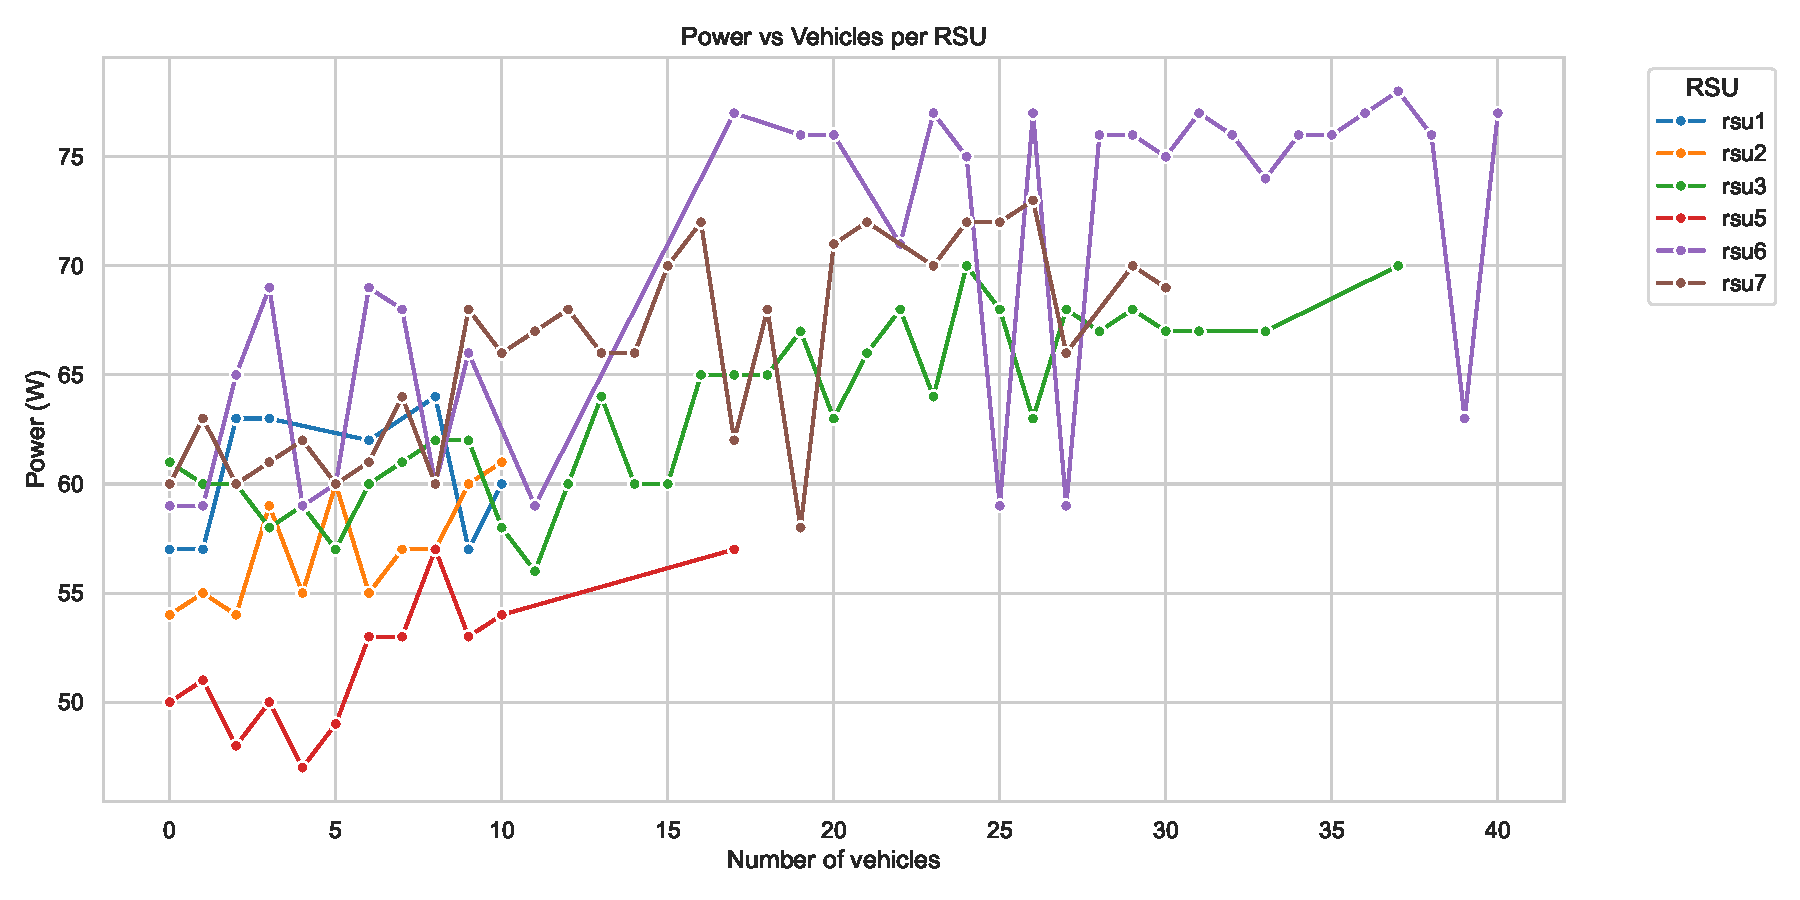
\includegraphics[width=1\columnwidth]{Figures/power_vehicles_rsu_maximums.pdf}
    \caption{Relationship between the number of vehicles and power consumption for each \gls{rsu}, showing how power usage increases with load and plateaus at maximum capacity.}
    \label{fig:exp1-figure}
\end{figure}